\documentclass{article}
\usepackage{graphicx}
\usepackage{subfig}
\usepackage{indentfirst}
\usepackage{amsmath}
\usepackage[verbose]{placeins} 
\usepackage{float}
\usepackage[top=2cm, bottom=2cm, right=2cm, left=2cm]{geometry}

% Title Page
\title{MAE 5730 Final Project \\
\large{Dynamic modeling of a spy zip-lining into a objective}}
\author{Mark Lohatepanont}




\begin{document}
\maketitle
\tableofcontents
\newpage
\section{Project Specification}
My project is to model the dynamics of a human taking a zipline through a arbitrarily defined course. The human, or “spy” in the context of this document consists of a 3-link body connected to a point mass. The point mass is representative of the zipline trolley, and the 3 links represent the head-neck connection, neck-waist connection and then waist to toe connection. \\

        
\begin{figure}[h]
    \centering
	\subfloat[\centering Anatomical Body]{{\includegraphics[width=5cm]{2anatomical_model} }}%
	\qquad
	\subfloat[\centering Sledge]{{\includegraphics[width=5cm]{point_mass} }}%
	\caption{Description of model components}%
	\label{fig:example}%
\end{figure}

A description of the 3 link connection is established visually above in Figure 1a where each of the links are described as rigid bodies which have their own lengths, masses, moments of inertia as well as their rotation as defined from the perpendicular of the previous link. For some more anatomical accuracy, the body’s joints will also act as torque dampers. 
This body’s head is then connected to a point mass which serves as the trolley and the forcing of the system that drives the spy through the course. 
Figure 1b describes the point mass setup with the first link (head connection) also being shown. As mentioned, the point mass has a forcing which will drive it through the course.
The course itself will be described by 3 distinct functions and is described visually in figure 3. Concretely, the 3 equations that compose the course are:
\begin{center}
	\begin{tabular}{c|c}
		Course Section & Function\\
		\hline
		1&$(\frac{x}{10}-3)^2+1$\\
		2&$\frac{-1}{10}+16$\\
		3&$-(\frac{x}{10}-12)^2+10$
	\end{tabular}
\end{center}

\begin{figure}[H]
	\centering
	\includegraphics[scale=0.5]{course_description}	
	\caption{Description of course}
\end{figure}

The spy’s trolley will be attached to the lines shown and follow the course. Where the start is at X = 0, and the end at X = 140.
The goal of the project is to develop the model and a visual representation of the system that can be plotted. An additional goal would be to find out how much forcing can be applied to the spy’s trolley to 
get them to the end of the course as quick as possible before the links loop upon themselves which will metaphorically mean that the spy has died and unsuccessfully made it to the end. 
\subsection{Global Free Body Diagram}
\begin{figure}[H]
	\centering
	\includegraphics[scale=0.5]{global_FBD_1_anno}	
	\caption{Global Free Body Diagram}
\end{figure}
Figure 3 depicts the general free body diagram. In minimal coordinates the trolley has 2 degrees of freedom in x and y, while the links are free to rotate with one degree of freedom each with their own angle. More accurate descriptions of the free body diagrams (FBD's) of each of the elements including the sledge and each link. For clarity the reaction forces have not been drawn, but they are shown in the individual FBD's in section 2.1.1. The constraints can be clearly defined as 2 non-conservative forces (Forcing and torque dampers) and 1 holonomic constraint (Positional Constraint from course).

\section{Equations of Motion}
\subsection{Differential Algebraic System of Equations Method (DAE)}
The setup consists of one force leading to a non-conservative force, one holonomic constraint coming from the course, and one non-holonomic constraint coming from the torque dampers. I will deal with the course's holonomic constraint by using constraint equations on the normal force interacting between the sledge and cart as well as the second derivative of the course's definition. For the torque damper, I’ll incorporate it into the angular moment balances to reduce the torque on the joints. Different sections of the course will be piece wised together. \\
\subsubsection{Free Body Diagrams}
To aid in the DAE method, I created free body diagrams for each of the bodies in my system. The bodies are the sledge, shown in Figure 4a, link 1, shwon in figure 4b, link 2 shown in figure 4c, and link 3 shown in figure 4d. Using these free body diagrams, I generated 11 Newton-Euler equations by performing Linear Momentum Balance (LMB) on the sledge, link 1, link 2 and link 3 in both the $\hat{i}$ and $\hat{j}$ coordinate frames along with 3 angular momentum balance (AMB) around the center of gravity's (CG) of link 1, link 2 and link 3. Along with these equations I also generated 8 constraint equations, 6 coming the constraints in the $\hat{i}$ and $\hat{j}$ in each of the three links. The last two constraints come from the holonomic constraints for the normal force which comes from the sledge interacting with the course.
\begin{figure}[h]
	\centering
	\subfloat[\centering Sledge FBD]{{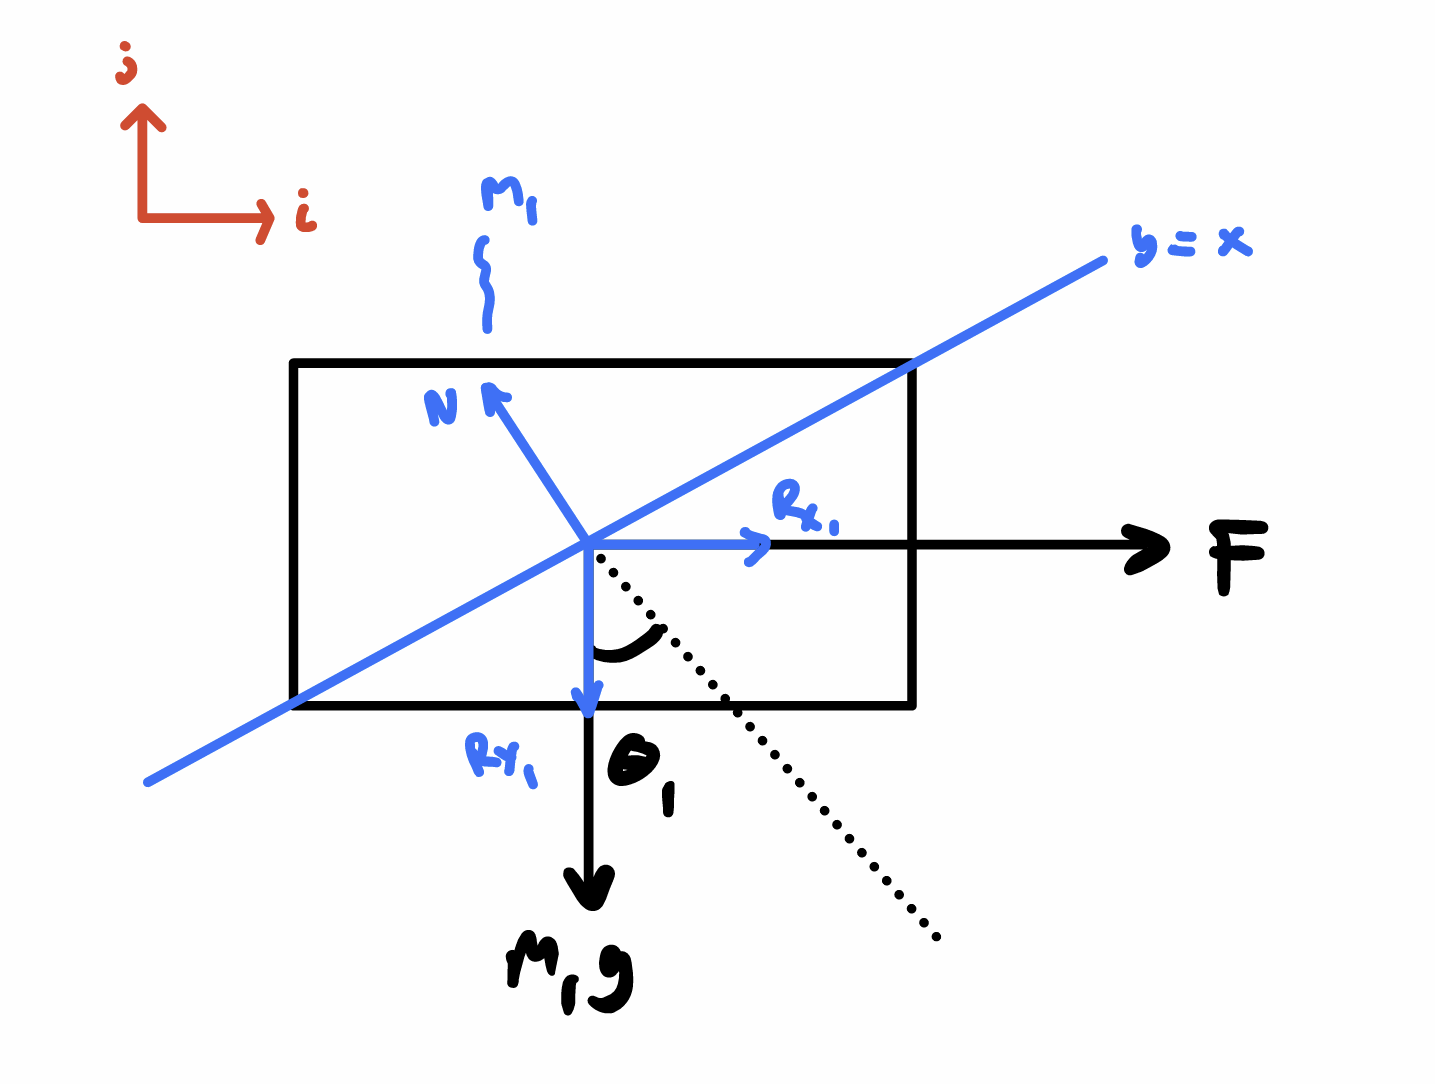
\includegraphics[width=7cm]{DAE_FBD_0} }}%
	\qquad
	\subfloat[\centering Link 1 FBD]{{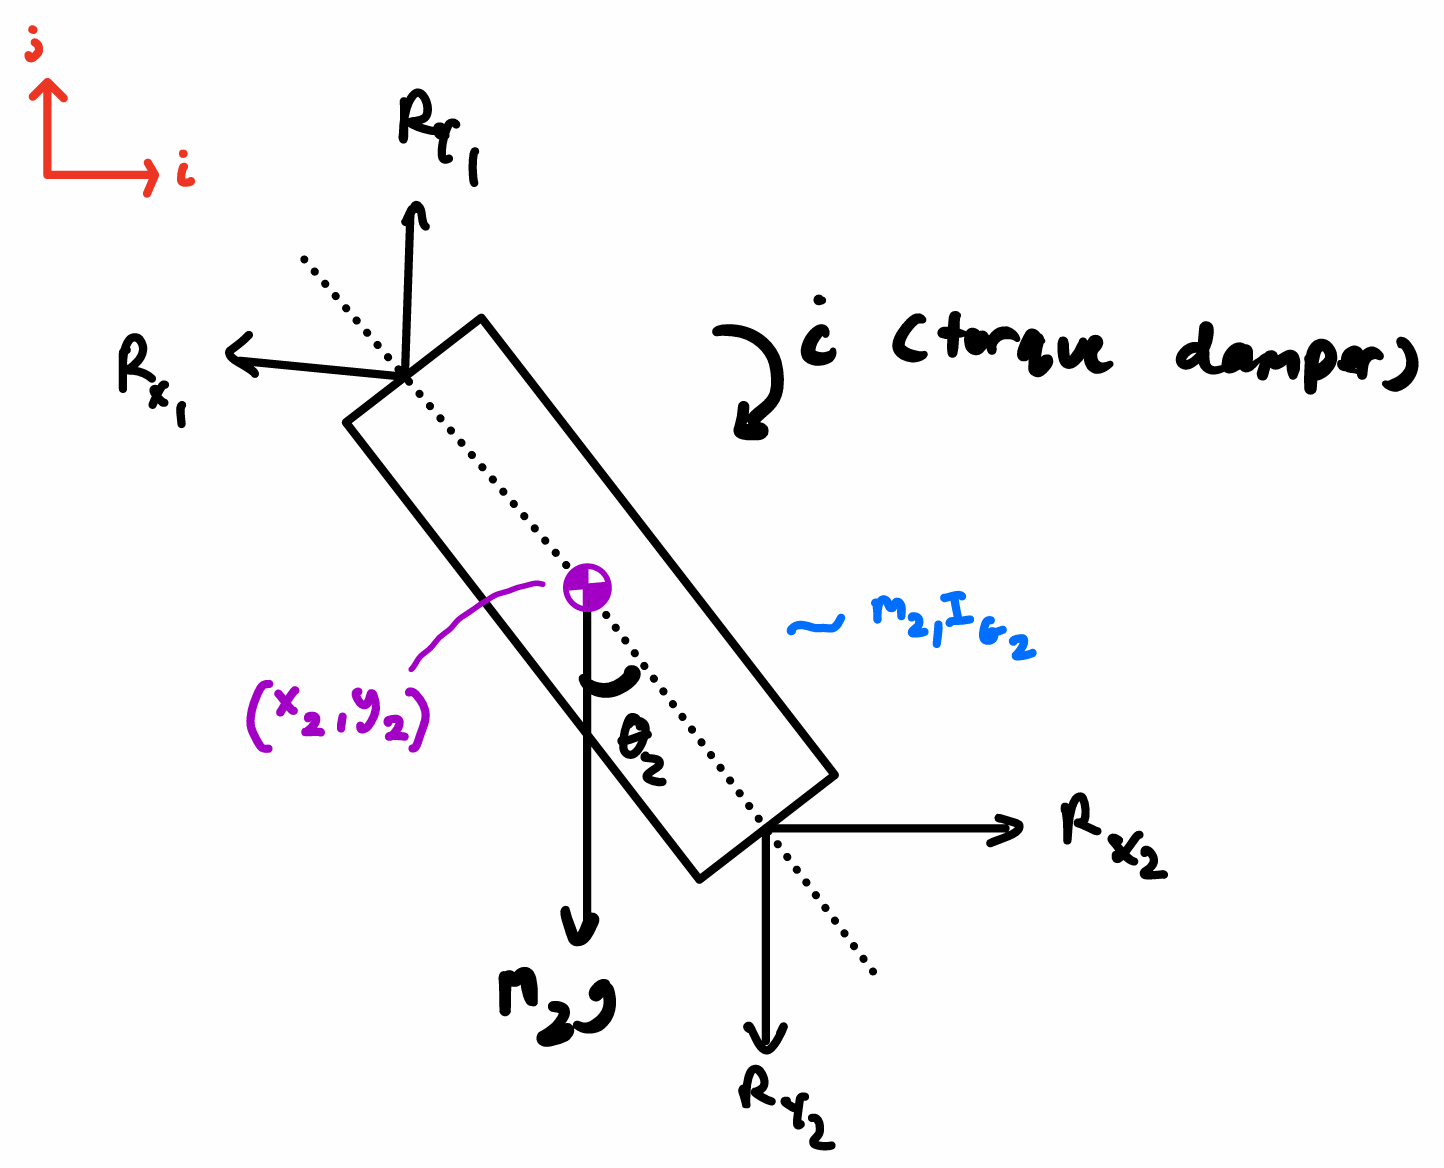
\includegraphics[width=7cm]{DAE_FBD_1} }}%\\
	\qquad
	\subfloat[\centering Link 2 FBD]{{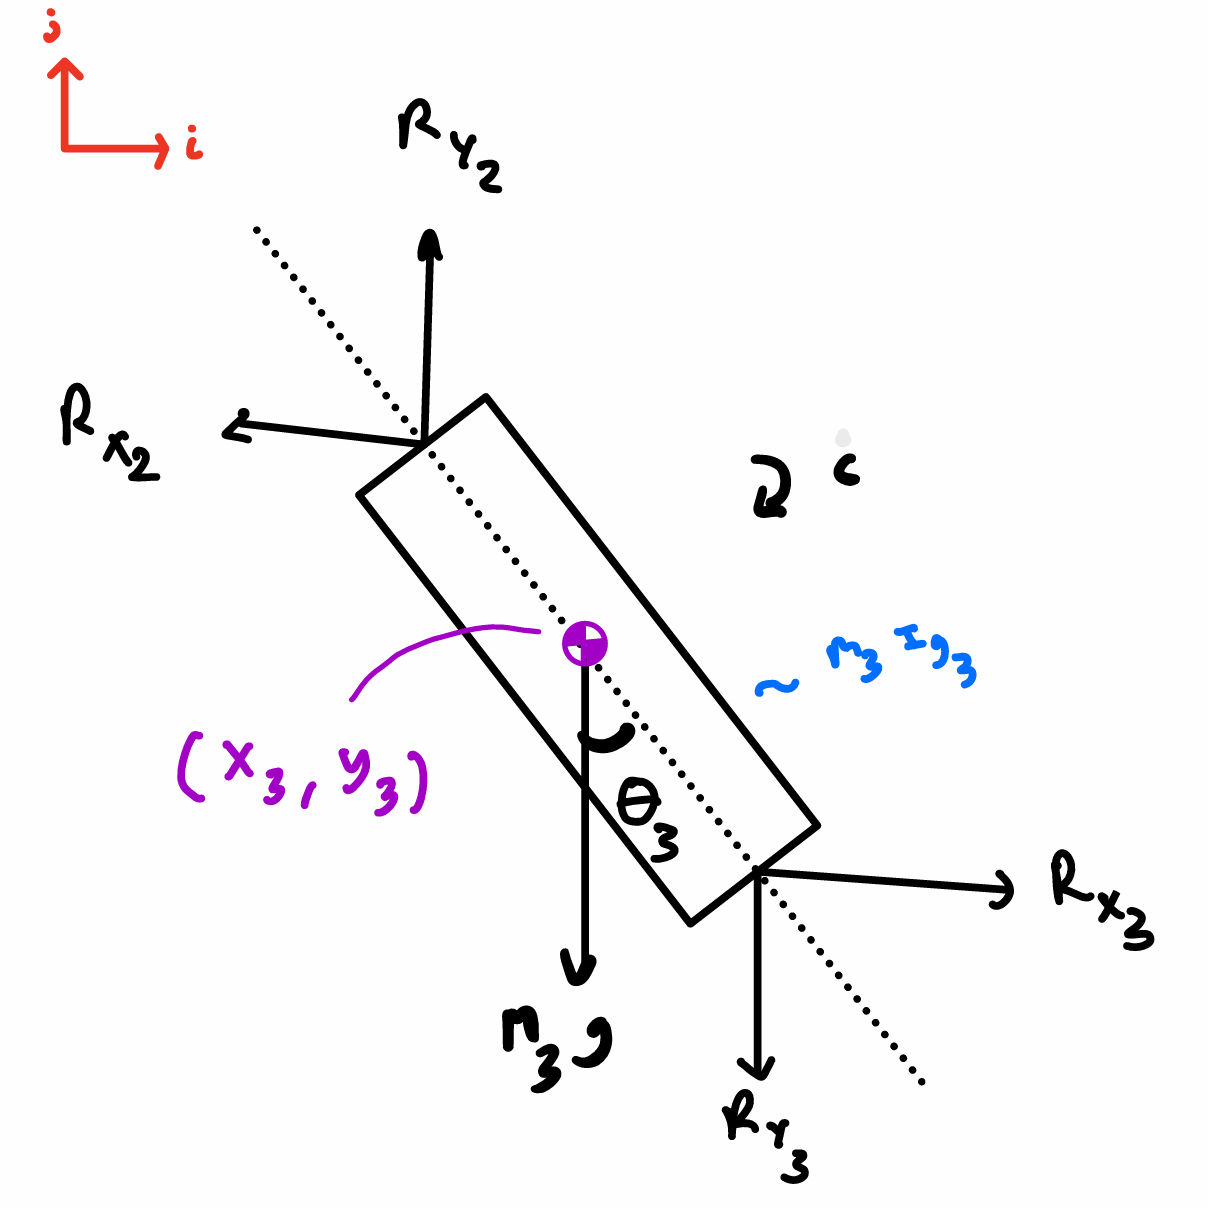
\includegraphics[width=7cm]{DAE_FBD_2} }}%\\
	\qquad
	\subfloat[\centering Link 3 FBD]{{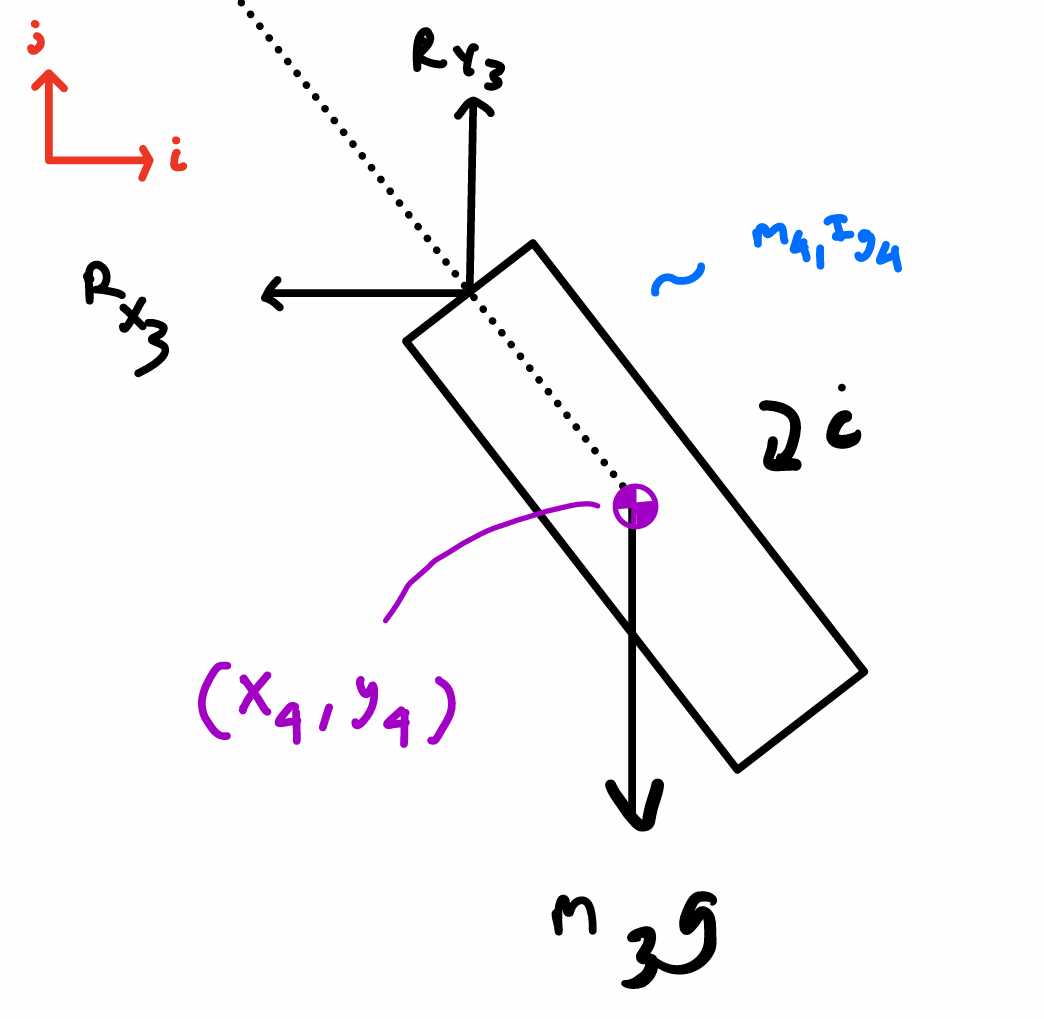
\includegraphics[width=7cm]{DAE_FBD_3} }}%\\
	\caption{Description of FBD model components}%
	\label{fig:example2}%
\end{figure}
\subsubsection{Equations}
From the free body diagrams and the DAE approach, a maximal coordinates approach is used with variables:
\begin{center}
	\begin{equation}
		q=\{x_1,y_1,x_2,y_2,\theta_1,x_3,y_3,\theta_2,x_4,y_4,\theta_3,R_{x_1},R_{y_1},R_{x_2},R_{y_2},R_{x_3},R_{y_3},F_{N_x}, F_{N_y} \}
	\end{equation} 
\end{center}
This leads to 19 unknowns, consistent with the number of equations listed above. By perform angular and linear momentum balances where applicable on the free body diagrams shown above the following equations are gained:

\hskip-0.0cm\begin{tabular}{c|c|c}
	n&Equation Origin&Equation\\
	\hline
	1&LMB in $\hat{i}$ on Sledge & $R_{x1} + F + F_{N_x} = m_1 \ddot{x}_1$\\
	2&LMB in $\hat{j}$ on Sledge & $-R_{y1} - m_1 g + F_{N_y} = m_1 \ddot{y}_1$\\
	\hline
	3&LMB in $\hat{i}$ on CG of Link 1&$-R_{x1} + R_{x2} = m_2 \ddot{x}_2$ \\
	4&LMB in $\hat{j}$ on Link 1&$R_{y1} - R_{y2} - m_2 g = m_2 \ddot{y}_2$ \\
	5&AMB on Link 1&$R_{x1} d_1 \cos(\theta_1) - R_{y1} d_1 \sin(\theta_1) + R_{x2} d_1 \cos(\theta_1) - R_{y2} d_1 \sin(\theta_1) - \dot{c}\dot{\theta_1}= I_{g1} \ddot{\theta}_1 $\\
	\hline
	6&LMB in $\hat{i}$ on Link 2&$-R_{x2} + R_{x3} = m_3 \ddot{x}_3$ \\
	7&LMB in $\hat{j}$ on Link 2&$R_{y2} - R_{y3} - m_3 g = m_3 \ddot{y}_3$ \\
	8&AMB on CG of Link 1&$R_{x2} d_2 \cos(\theta_2) - R_{y2} d_2 \sin(\theta_2) + R_{x3} d_2 \cos(\theta_2) - R_{y3} d_2 \sin(\theta_2) - \dot{c}\dot{\theta_2} = I_{g2} \ddot{\theta}_2 $\\
	\hline
	9&LMB in $\hat{i}$ on Link 2&$ -R_{x3} = m_4 \ddot{x}_4$ \\
	10&LMB in $\hat{j}$ on Link 2&$R_{y3} - m_4 g = m_4 \ddot{y}_4$ \\
	11&AMB on CG of Link 1&$R_{x3} d_3 \cos(\theta_3) - R_{y3} d_3 \sin(\theta_3) = I_{g3} \ddot{\theta}_3 - \dot{c}\dot{\theta_3}$\\
	\hline
	12&Constraint for $\hat{i}$ in link 1&$x_2 = x_1(t) + d_1 \sin(\theta_1(t))$\\
	13&Constraint for $\hat{j}$ in link 1&$y_2 = y_1(t) - d_1 \cos(\theta_1(t))$\\
	14&Constraint for $\hat{i}$ in link 2&$x_3 = x_1(t) + 2 d_1 \sin(\theta_1(t)) + d_2 \sin(\theta_2(t))$\\
	15&Constraint for $\hat{j}$ in link 2&$y_3 = y_1(t) - 2 d_1 \cos(\theta_1(t)) - d_2 \cos(\theta_2(t))$\\
	16&Constraint for $\hat{i}$ in link 3&$x_4 = x_1(t) + 2 d_1 \sin(\theta_1(t)) + 2 d_2 \sin(\theta_2(t)) + d_3 \sin(\theta_3(t))$\\
	17&Constraint for $\hat{j}$ in link 3&$y_4 = y_1(t) - 2 d_1 \cos(\theta_1(t)) - 2 d_2 \cos(\theta_2(t)) - d_3 \cos(\theta_3(t))$
\end{tabular}



The last two equations depend on the stage of the course and varies between the courses functions. The constraint is developed from the normal force acting on the sledge with equation $F_{N_x} + F_{N_y}\frac{dy}{dx}=0$. The second constraint comes from the double derivative of the function putting a constraint linking $\ddot{y}$ and $\ddot{x}$. The course functions and their constraints are listed below
\begin{center}
	\begin{tabular}{c|c|c}
		Function&Constraint 1&Constraint 2\\
		\hline
		$(\frac{x}{10}-3)^2+1$&$F_{N_x}+(\frac{x}{50}-\frac{3}{5})F_{N_y}=0$&$\ddot{y}=\frac{\dot{x}^2}{50} + \frac{\left(\frac{x}{10} - 3\right) \ddot{x}}{5}$\\
		$\frac{-1}{10}+16$&$F_{N_x}-\frac{F_{N_y}}{10}=0$&$\ddot{y}=\frac{-1}{10}\ddot{x}$\\
		$-(\frac{x}{10}-12)^2+10$&$F_{N_x}+(\frac{12}{5}-\frac{x}{50})F_{N_y}=0$&$\ddot{y}=-\frac{\dot{x}^2}{50}-\frac{\frac{x}{10}-12}{5}\ddot{x}$\\
	\end{tabular}
\end{center}
These 19 equations are then entered into matlab and solved for each of the maximal coordinates. 
\subsubsection{Initial Conditions}
When entering a zipline, I felt like most people try to enter them as straight as possible. So I will also model the individual as being straight at the beginning of the course. Since the sledge is providing forcing, I will also not add any initial velocities to any of the coordinates. Further, for simulation setup, I defined each length of $d_1=d_2=d_3=5$ and the masses $m_1=30, m_2=15,m_3=5,$ and $m_4 = 2$. To further summarize the state variables used for the simulation, out of the 19 maximal coordinates, only 3 will be non-zero, this is summarized below:
\begin{center}
	\begin{tabular}{c|c||c|c||c|c}
		Coordinate&Initial Condition&Coordinate&Initial Condition&Coordinate&Initial Condition\\
		\hline
		$x_1$&0&$y_1$&10&&\\
		$x_2$&0&$y_2$&5&$\theta_1$&0\\
		$x_3$&0&$y_3$&0&$\theta_2$&0\\
		$x_4$&0&$y_4$&-5&$\theta_3$&0\\
	\end{tabular}
\end{center}
Other conditions were a forcing of $F = 100N$ and torque campers with $c = -1$.

\subsection{Euler-Lagrange Method}
\subsubsection{Constraints}
The setup consists of one force leading to a non-conservative force, one holonomic constraint coming from the course, and one non-holonomic constraint coming from the torque dampers. I will deal with the holonomic constraint by using a Lagrange multiplier.  An example of how I deal with the trivial case of in the course where $y=-\frac{1}{10}x+16$, the holonomic constraint becomes $\dot{y}=\frac{1}{10}\dot{x}$, with the differential form being $fdt=dy-\frac{dx}{10}=0$, which leads to the Lagrange multipliers of $f_x=1$,$f_y=1$. These can then be incorporated into the equations of motion calculations.  For the torque damper, I’ll use the Raleigh dissipation equation to reduce the torque on the joints. Different sections of the course will be piece wised together. \\
For each of the three stages of the course using a holonomic constraint the differential form as well as the constraint is described in the following table:
\begin{center}
\begin{tabular}{c|c|c|c|c}
	Function&Differential Form&$f_x$&$f_y$&Double Derivative Constraint\\
	\hline
	$(\frac{x}{10}-3)^2+1$&$dy-\frac{\left(\frac{x}{10} - 3\right)}{5} dx=0$&$-\frac{\left(\frac{x}{10} - 3\right)}{5}$&1&$\ddot{y}=\frac{\dot{x}^2}{50} + \frac{\left(\frac{x}{10} - 3\right) \ddot{x}}{5}$\\
	$\frac{-1}{10}+16$&$dy+\frac{1}{10}dx$&$\frac{1}{10}$&1&$\ddot{y}=\frac{-1}{10}\ddot{x}$\\
	$-(\frac{x}{10}-12)^2+10$&$dy+\frac{\frac{x}{10}-12}{5}dx=0$&$\frac{\frac{x}{10}-12}{5}$&1&$\ddot{y}=-\frac{\dot{x}^2}{50}-\frac{\frac{x}{10}-12}{5}\ddot{x}$\\
\end{tabular}
\end{center}
\subsubsection{Lagrange Equations}
The generalized coordinates are chosen as the minimal set of coordinates $q_i = \{ x,y,\theta_1,\theta_2,\theta_3 \} $. The Lagrange equations come from the kinetic and potential energy. The kinetic energy can be found by summing up the kinetic energy of the sledge and each of the links combined with the rotational energy of each of the links. This is loosely described below in equation 1.
\begin{equation}\label{Kinetic Energy Equation}
	E_k = \frac{1}{2} \left( m_1 v_1^2 + m_2 v_2^2 + I_{g1} \dot{\theta}_1^2 + m_3 v_3^2 + I_{g2} \dot{\theta}_2^2 + m_4 v_4^2 + I_{g3} \dot{\theta}_3^2 \right) 
\end{equation}
The velocities $v1, v2, v3,$ and $v4$ can be found in the generalized coordinates by the following equations described in 2.:
\begin{equation}
	\hskip-0.0cm\begin{split}
		v_1 = \sqrt{\dot{x}_1^2 + \dot{y}_1^2} \\
		v_2 = \sqrt{\left( \dot{x}_1 + d_1 \dot{\theta}_1 \cos(\theta_1) \right)^2 + \left( \dot{y}_1 - d_1 \dot{\theta}_1 \sin(\theta_1) \right)^2}\\
		v_3 = \sqrt{\left( \dot{x}_1 + d_1 \dot{\theta}_1 \cos(\theta_1) + d_2 \dot{\theta}_2 \cos(\theta_2) \right)^2 + \left( \dot{y}_1 - d_1 \dot{\theta}_1 \sin(\theta_1) - d_2 \dot{\theta}_2 \sin(\theta_2) \right)^2}\\		
		v_{g4} = \sqrt{\left( \dot{x}_1 + 2d_1 \cos(\theta_1) \dot{\theta}_1 + 2d_2 \cos(\theta_2) \dot{\theta}_2 + d_3 \cos(\theta_3) \dot{\theta}_3 \right)^2 + \left( \dot{y}_1 + 2d_1 \sin(\theta_1) \dot{\theta}_1 + 2d_2 \sin(\theta_2) \dot{\theta}_2 + d_3 \sin(\theta_3) \dot{\theta}_3 \right)^2}		
	\end{split}
\end{equation}
Finally, the potential energy is defined in 3 as the heights of the center of gravity of the point mass and each link measured from the datum where $y=0$:
\begin{equation}
	\begin{split}
			E_p = g ( m_1 y_1 + m_2 \left( y_1 - d_1 \cos(\theta_1) \right) + m_3 \left( y_1 - d_1 \cos(\theta_1) - d_2 \cos(\theta_2) \right) \\
		+ m_4 \left( y_1 - d_1 \cos(\theta_1) - d_2 \cos(\theta_2) - d_3 \cos(\theta_3) \right) )	
	\end{split}
\end{equation}
The Lagrangian is then defined as $\mathcal{L} = E_k - E_p$. This is too long, and will not be shown here but can be inspected in the appendix 6.1.
An additional section to the Lagrangian is the Lagrangian generalized non-conservative forces terms. These terms accounts for the constraints in the course as well as the forcing and damping in the system. The forcing is represented by a positive $x$ direction value of 100N, the torque dampers are represented by a value equal to $-c\dot{\theta_n}$ in each of the thetas, and the holonomic constraint from the course as mentioned in the table from 2.1.1 leads to the lagrange multipliers that appear in the $x$ and $y$ terms. The generalized non-conservative force terms exist for each of the 5 generalized coordinates and differ for each of the three course sections. The terms summarized as a vector with 5 components with the component 1 representing non-conservative forces in $x$, component 2 in $y$, component 3 in $\theta_1$, component 4 in $\theta_2$ and component 5 in $\theta_3$. This is shown in the table below as the Q vector corresponding to each course section:
\begin{center}
	\begin{tabular}{c|c|c}
		Course Section& Function & Generalized non-conservative forces Q terms\\
		\hline
		1&$(\frac{x}{10}-3)^2+1$ & $Q_1$ = [ $100 - \frac{1}{5} \left( \frac{x_1}{10} - 3 \right) \lambda$, $\lambda$, $c\dot{\theta_1}$,  $c\dot{\theta_2}$,  $c\dot{\theta_3}$ ]\\
		2&$\frac{-1}{10}+16$& $Q_2$ = [ $100-\frac{1}{10} \lambda$, $\lambda$, $c\dot{\theta_1}$,  $c\dot{\theta_2}$,  $c\dot{\theta_3}$ ]\\
		3&$-(\frac{x}{10}-12)^2+10$&$Q_3$ = [ $100 + \frac{1}{5} \left( \frac{x_1}{10} - 12 \right) \lambda$, $\lambda$, $c\dot{\theta_1}$,  $c\dot{\theta_2}$,  $c\dot{\theta_3}$ ]\\
		
	\end{tabular}
\end{center}
To obtain the equations of motion the following is used for each of the conditions where in $Q_n[x]$, $n$ represents the stage of the equation and $x$ represents the index of the generalized coordinate to be used. Given that the full definitions are too long, I will only provide the generalized form with generalized coordinates substituted. For clarity, I will also substitute in the non-generalized force terms for the first course section:
\begin{center}
	\begin{tabular}{c|c|c}
		Generalized Coordinate & EL equation &First Course Section\\
		\hline
		$x_1$ & $\frac{d}{dt}\frac{\partial{\mathcal{L}}}{\partial{\dot{x_1}}}-\frac{\partial{\mathcal{L}}}{\partial{x_1}}=Q_n[1]$&$Q_1[1] = 100 - \frac{1}{5} \left( \frac{x_1}{10} - 3 \right) \lambda$\\
		$y_1$ & $\frac{d}{dt}\frac{\partial{\mathcal{L}}}{\partial{\dot{y_1}}}-\frac{\partial{\mathcal{L}}}{\partial{y_1}}=Q_n[2]$&$Q_1[2] = \lambda$\\
		$\theta_1$ & $\frac{d}{dt}\frac{\partial{\mathcal{L}}}{\partial{\dot{\theta_1}}}-\frac{\partial{\mathcal{L}}}{\partial{\theta_1}}=Q_n[3]$ & $Q_1[3] = c\theta_1$	\\		
		$\theta_2$ & $\frac{d}{dt}\frac{\partial{\mathcal{L}}}{\partial{\dot{\theta_2}}}-\frac{\partial{\mathcal{L}}}{\partial{\theta_2}}=Q_n[4]$& $Q_1[4] = c\theta_2$	\\
		$\theta_3$ & $\frac{d}{dt}\frac{\partial{\mathcal{L}}}{\partial{\dot{\theta_3}}}-\frac{\partial{\mathcal{L}}}{\partial{\theta_3}}=Q_n[5]$& $Q_1[5] = c\theta_3$	\\
	\end{tabular}
\end{center}
For my implementation I used the Jacobian representation to calculate the equations of motion and saved them to functions in matlab. 
\subsubsection{Initial Conditions}
Following the same rules as dictates in the DAE method analysis section 2.1.3, the EL equations will follow a similar basis where the individual is connected to the course in a vertical setup. Similarly, for simulation setup, I defined each length of $d_1=d_2=d_3=5$ and the masses $m_1=30, m_2=15,m_3=5,$ and $m_4=2$. For the state variables used in the minimal coordinates version of this problem the initial conditions for the velocities are all 0 and the positions for the EL method is:
\begin{center}
	\begin{tabular}{c|c}
		Coordinate&Initial Condition\\
		\hline
		$x_1$&0\\
		$y_1$&10\\
		$\theta_1$&0\\
		$\theta_2$&0\\
		$\theta_3$&0
	\end{tabular}
\end{center}
Other conditions were a constant forcing of $F = 100N$ and torque campers with $c = -1$.
\newpage
\section{Still Frames}
Figure's 5 and 6 illustrate still frames taken from two sections of the course, where figure a refers to a frame from the DAE method and figures b refer to a frame from the EL method. Figure 5 comes from the start of the section of the course where $x = 0$ along the function $(\frac{x}{10}-3)^2+16$, while figure 6 comes from an earlier section of the course where $x=20$ along the same function. The initial conditions for all cases I tested started with the human swinging off the sledge (red) being completely upright, with the values $\theta_1 = \theta_2 = \theta_3=0$ No initial forcing is present except for the forcing of the sledge. The forcing of the sledge is variable between each of the stages but for the following simulations all course stages had the same forcing at $F = 100N$.

\begin{center}
	\begin{figure}[H]
		\centering
		\subfloat[\centering DAE Still Frame]{{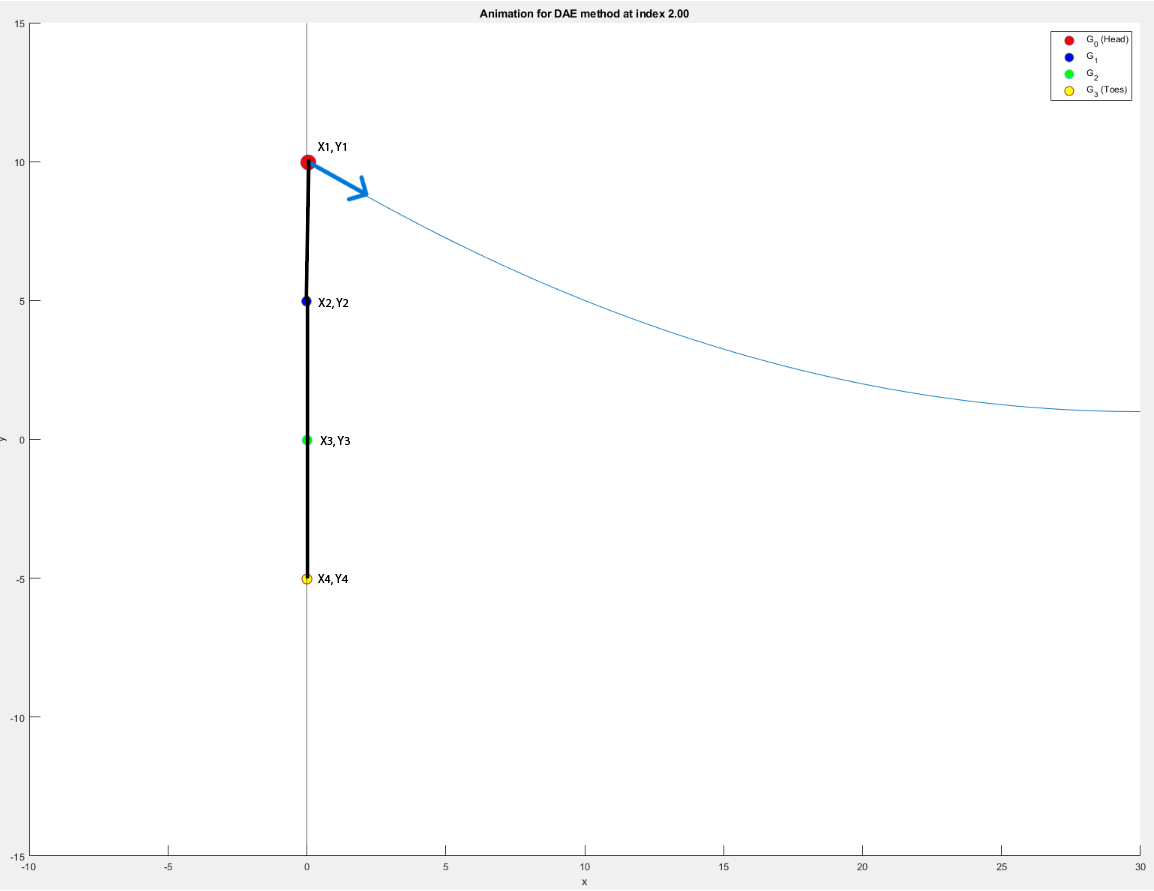
\includegraphics[width=10cm]{DAE_SF_2_anno} }}%\\
		
		\subfloat[\centering EL Still Frame]{{\includegraphics[width=10cm]{EL_SF_2_anno} }}%\\
		\caption{Still frames of the DAE and EL method at $x=0$, at the start of the simulation}%
		\label{fig:example3}%
	\end{figure}
\end{center}


\begin{center}
	\begin{figure}[H]
		\centering
		\subfloat[\centering DAE Still Frame]{{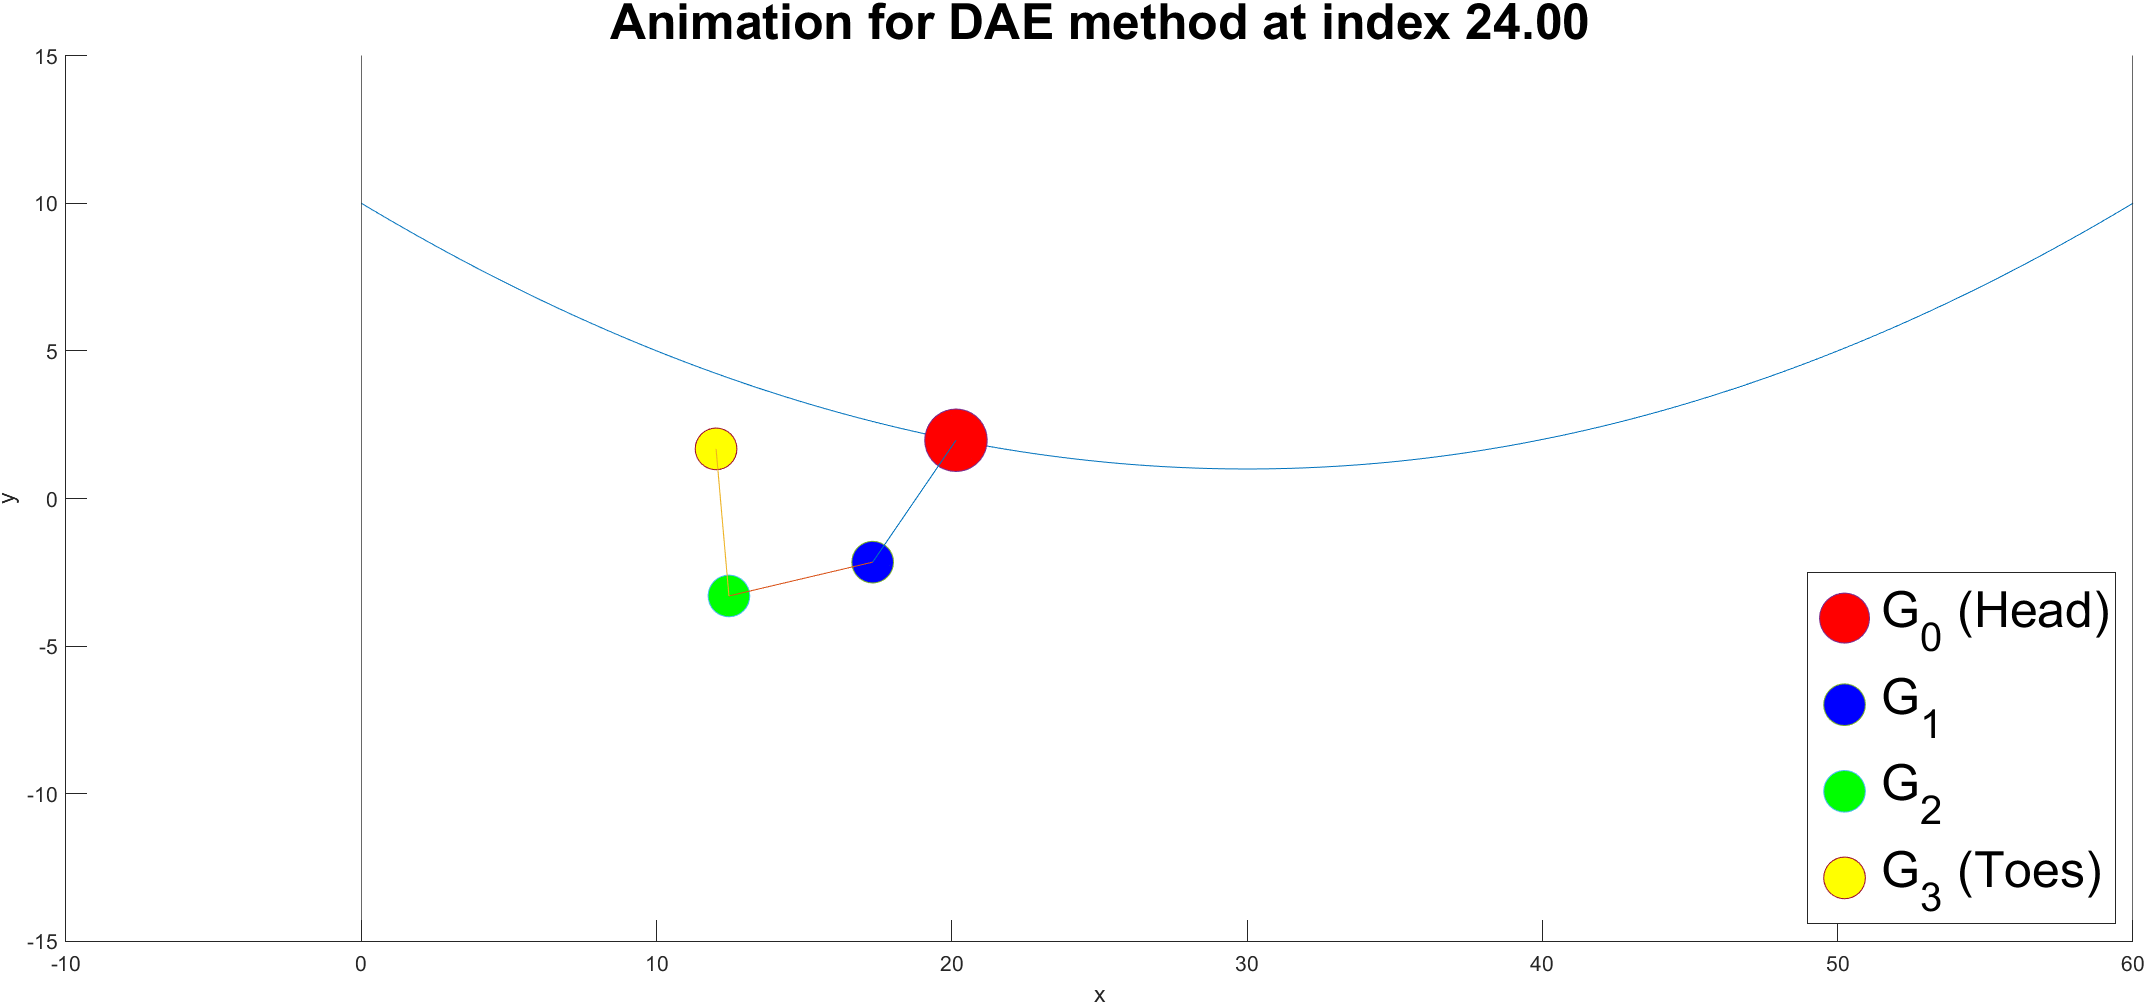
\includegraphics[width=10cm]{DAE_SF_1} }}%\\
		
		\subfloat[\centering EL Still Frame]{{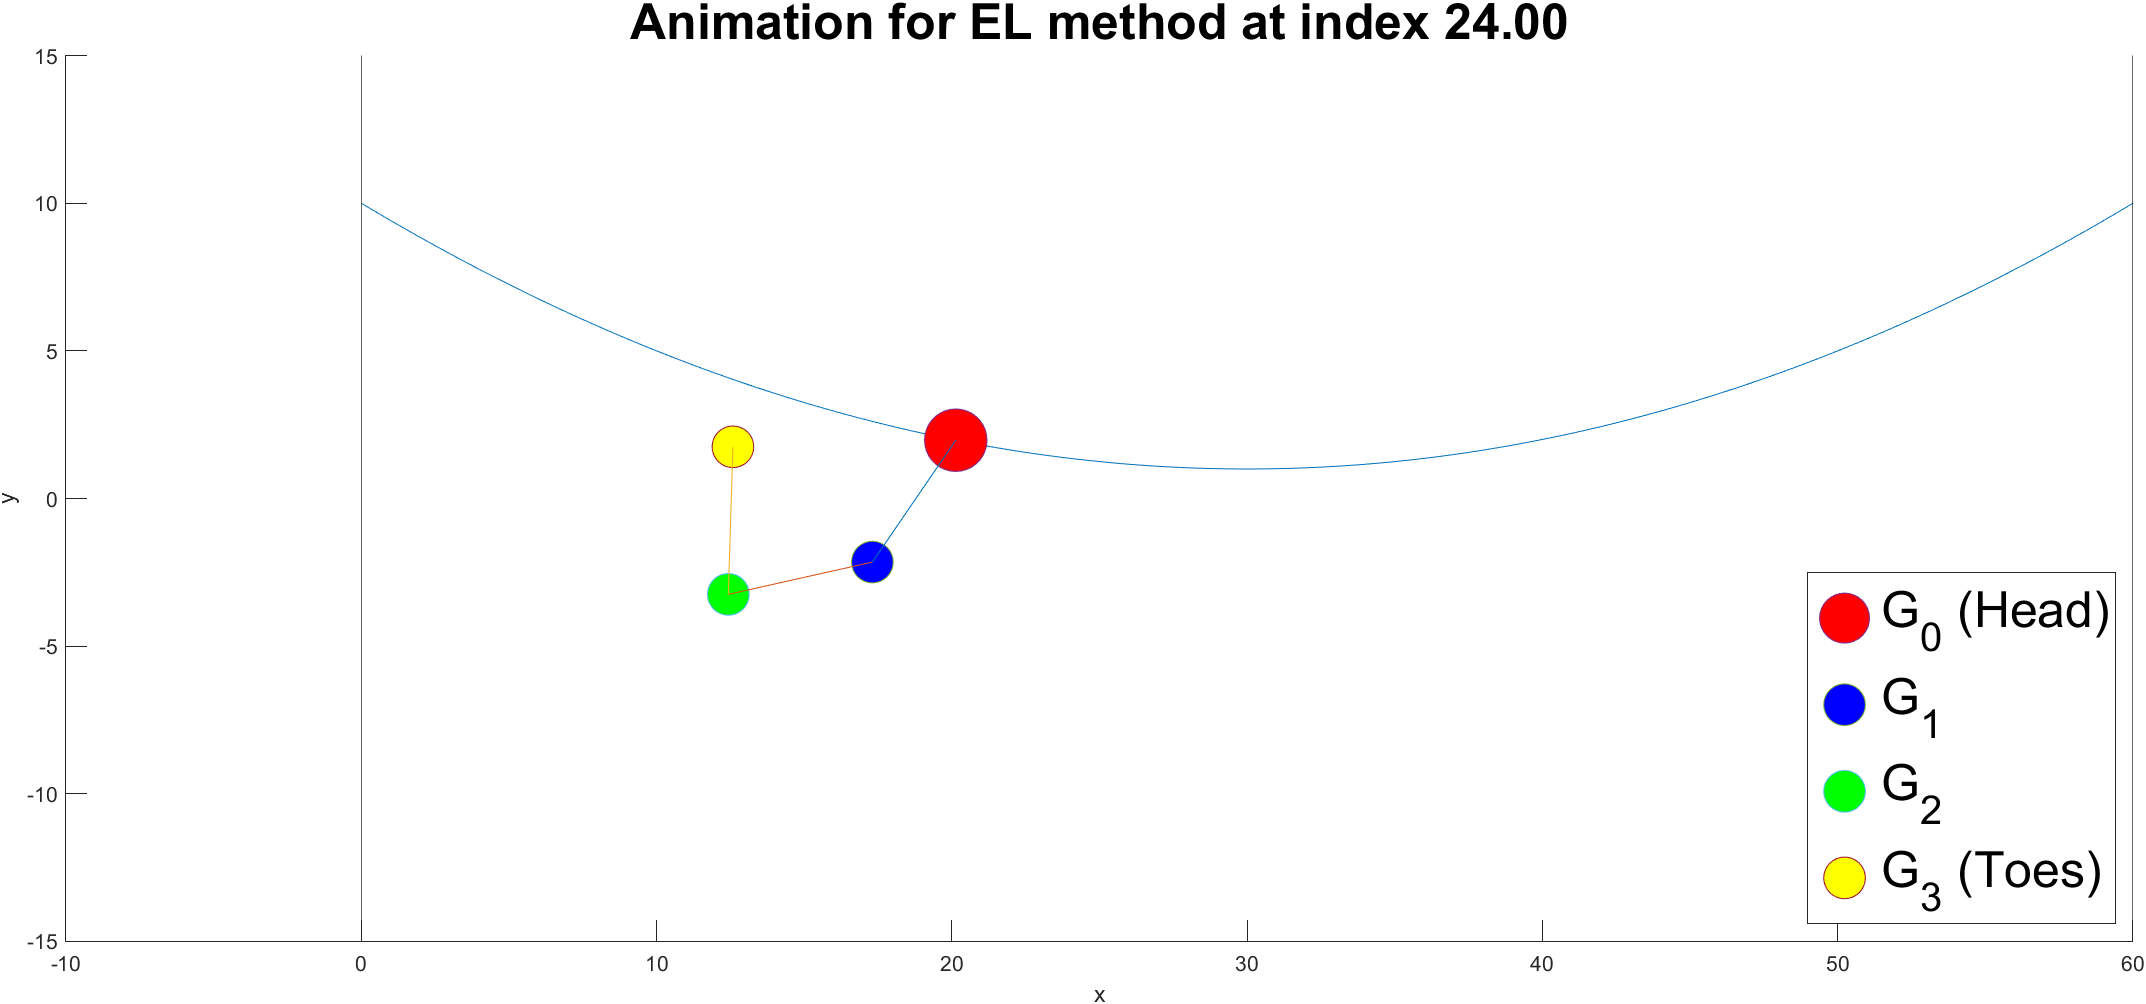
\includegraphics[width=10cm]{EL_SF_1} }}%\\
		\caption{Still frames of the DAE and EL method at $x=20$}%
		\label{fig:example4}%
	\end{figure}
\end{center}


\section{Trajectory Plots}
\begin{center}
	\begin{figure}[H]
		\centering
		\subfloat[\centering DAE Trajectory]{{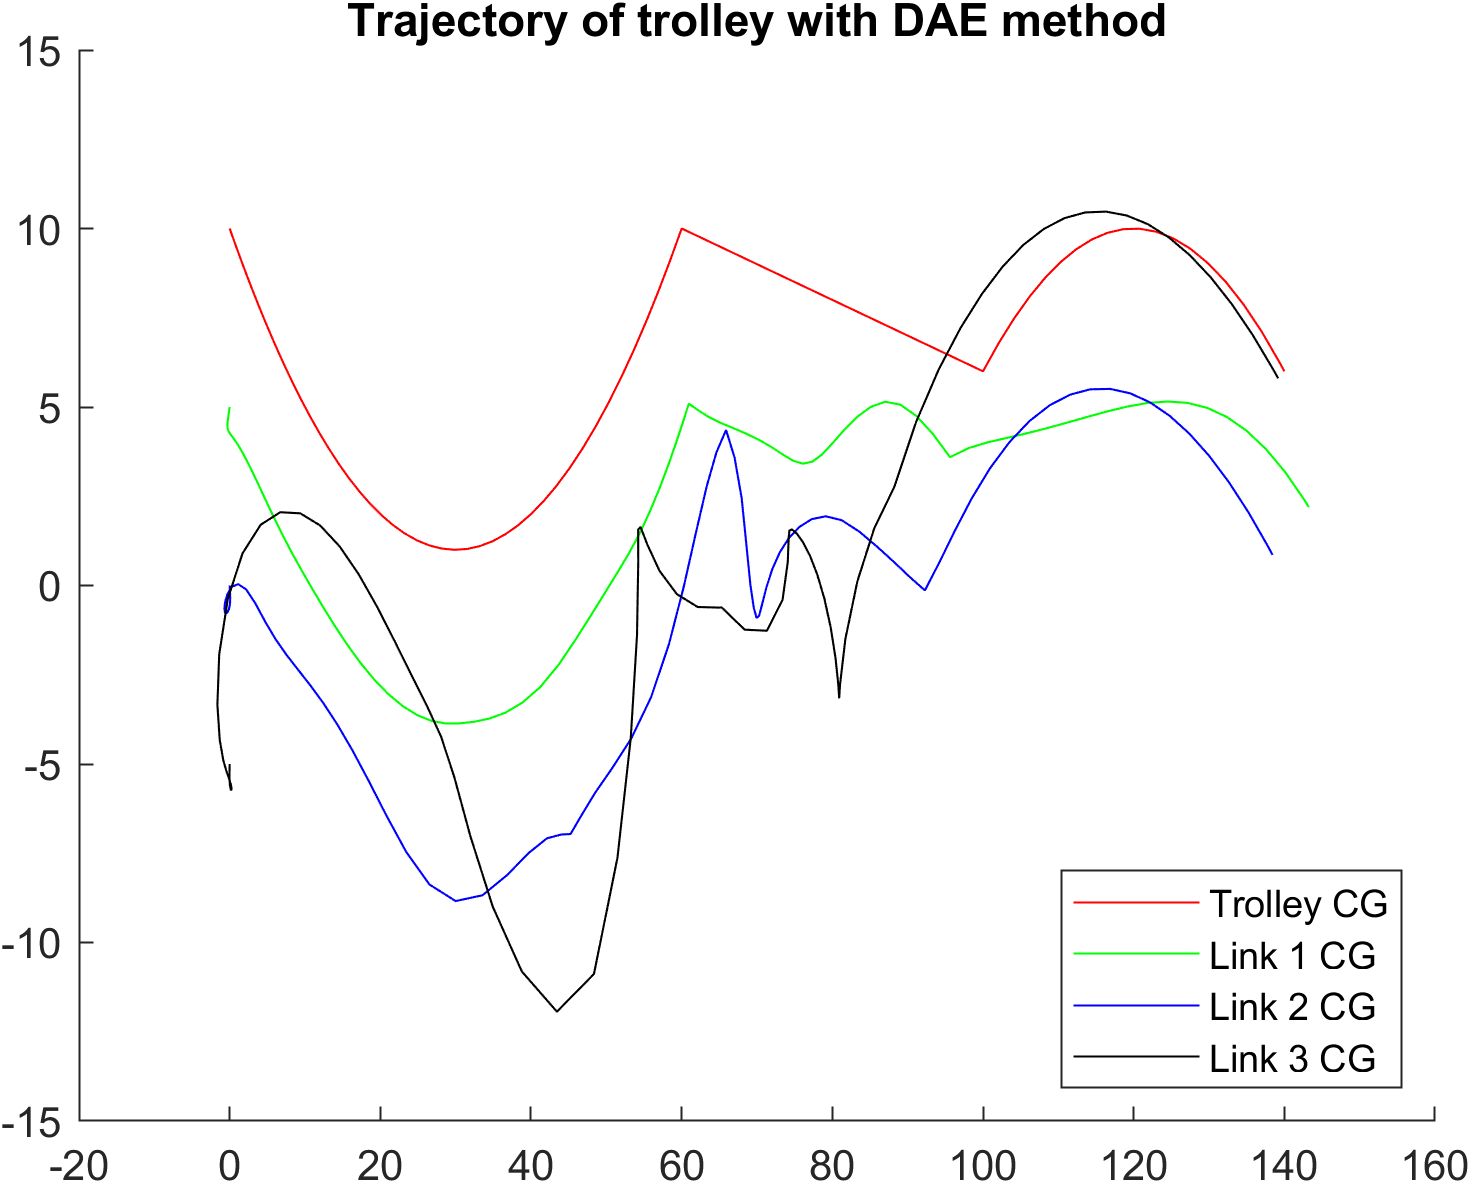
\includegraphics[width=8cm]{Traj_DAE_0} }}%\\
		
		\subfloat[\centering EL Trajectory]{{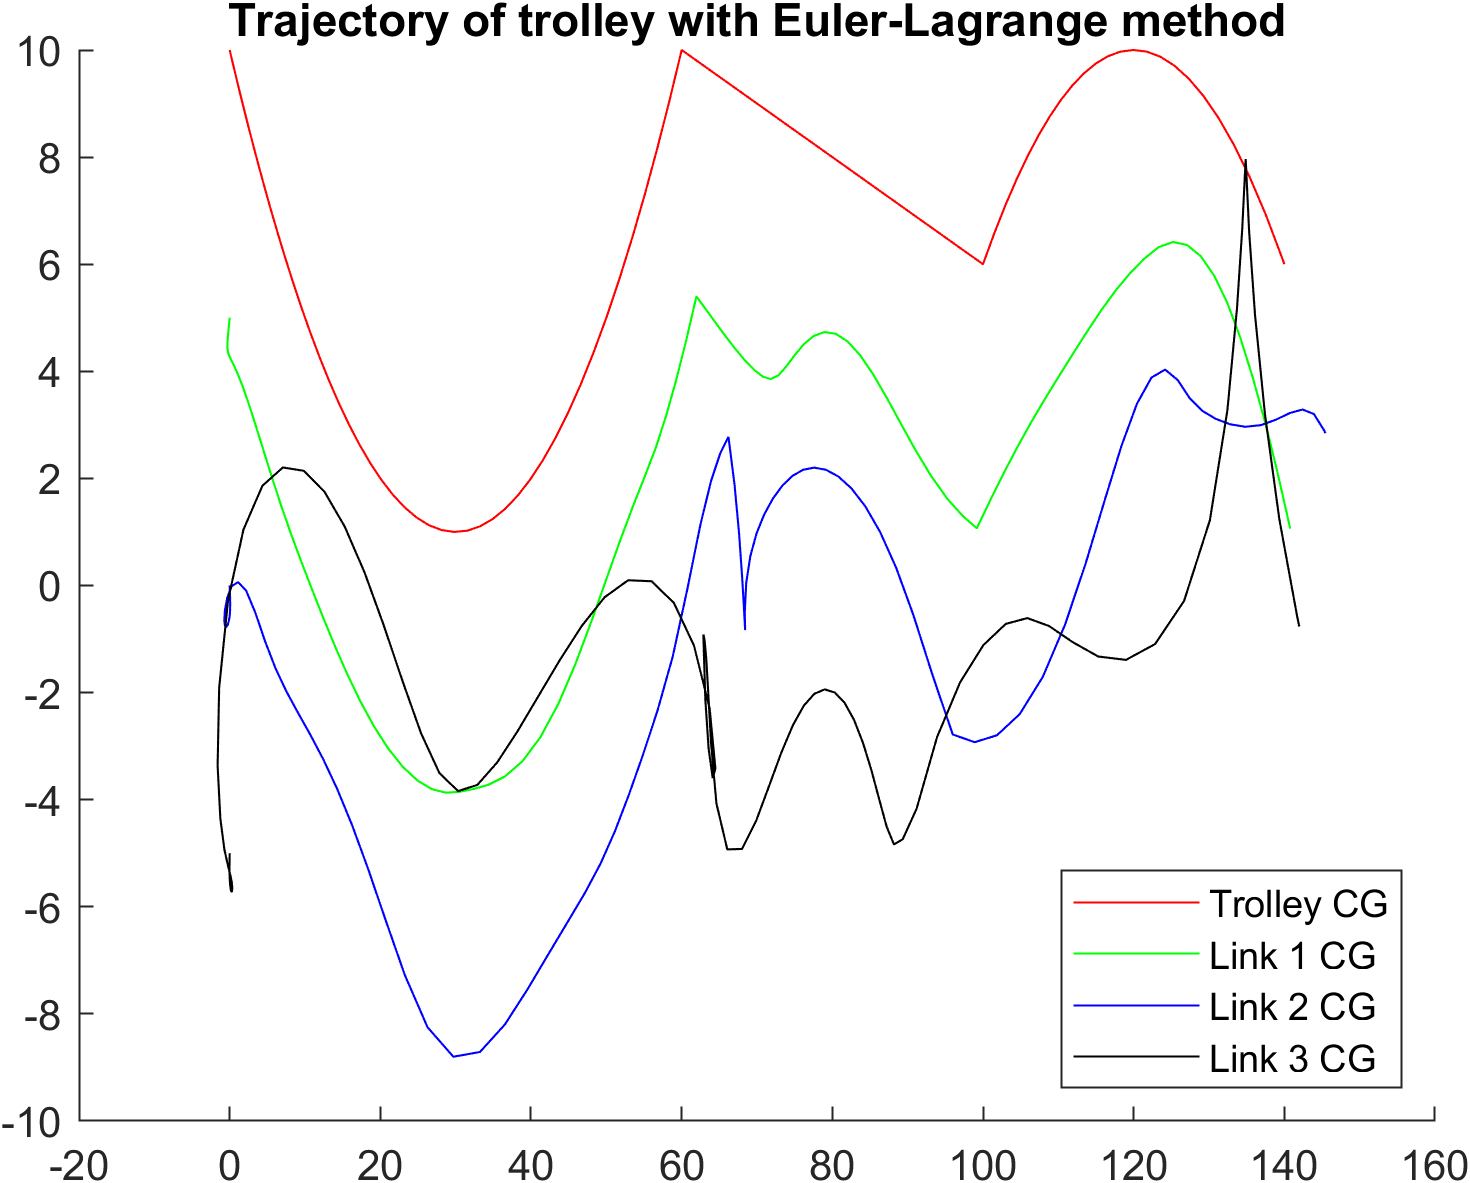
\includegraphics[width=8cm]{Traj_EL_0} }}%\\
		\caption{Trajectory plots along the entire course for DAE and EL methods}%
		\label{fig:example5}%
	\end{figure}
\end{center}
For a more global view of the entire course, I have also included trajectory plots of where the CG of the point mass and each link are across the entire course.
\section{Discussion}
The results of this project demonstrate the effectiveness of modeling a multi-link system traversing a zipline course using both the Euler-Lagrange (EL) and Differential Algebraic Equations (DAE) approaches.

The DAE approach was easier to handle the dynamic constraints of the system. By using maximal coordinates, it effectively incorporated the holonomic and non-holonomic constraints directly into the equations of motion. This streamlined the simulation process, particularly for sections of the course with abrupt changes in the slope or curvature. The still frames captured from the DAE simulation illustrate smooth transitions along the course, aligning closely with the expected physical behavior of the system. However, the computational cost of managing these constraints was not negligible, particularly as the number of variables increased and this manifested in a slightly longer runtime.

The EL approach, while easier to develop the basic equations of motion through energy-based principles, required additional effort to handle the constraints via Lagrange multipliers. Despite this, the EL trajectory demonstrated consistent results, indicating that the method is probably better suited systems with clearly defined energy relationships and smooth constraint transitions.

One notable finding was the impact of forcing on the system’s stability and traversal time. Higher forces accelerated the spy along the course but also increased the likelihood of link looping, particularly in tighter curves. Adjusting the forcing function for each section of the course could mitigate these issues, ensuring a balance between speed and stability. This presents a clear area for optimization in future iterations of the model.

The transition points between course segments also highlighted the limitations of the current setup. The problem with the current setup is that at the boundary conditions where the course changes, the final state that the system is in from the previous state did not follow the constraints of the next section. This required altering of the state variables so that the final state from the previous section obeyed the next sections constraints. Discussing the other constraints in the system I think while they were sufficient for this project, incorporating additional factors, such as cable elasticity or environmental effects, would enhance the realism of the simulation. Furthermore, refining the damping properties of the joints to better represent human-like motion could offer deeper insights into the dynamics of the system.

A discussion about the trajectory plots, the DAE and EL methods differ in their trajectories. While at the beginning, the motion closely matches each other, there seems to be differences towards the later section of the course. This interestingly only occurred when I added the torque dampers and signifies there may be a issue with my implementation. However, even then, the current setup seems to match up closely with each other if you inspect only the general shapes the trajectory takes. For example in the middle section there exist two peaks before a third peak occurs in the last section. This is present in both of the trajectory plots and indicates that the bug perhaps is minor. 

To extend the discussion to energy, I have included an energy plot in figure 8. The energy plot shows that the system is non-conservative, with kinetic energy (KE) increasing significantly due to external forcing while potential energy (PE) remains relatively constant. This makes sense as the sledge has external forcing and is driving the system forward, adding energy and breaking conservation. Additionally, the torque dampers at the joints dissipate mechanical energy, further contributing to the non-conservation of energy. The relatively flat PE suggests that vertical motion has a minimal effect on the system’s energy dynamics, consistent with a primarily horizontal trajectory of the system where the $Y$ values of the system only ever range from 10 and -12. Overall, the observed energy behavior reflects the influence of external forcing as well as damping, which aligns with the non-conservative assumptions of the modeled system.
\begin{center}
	\begin{figure}[H]
		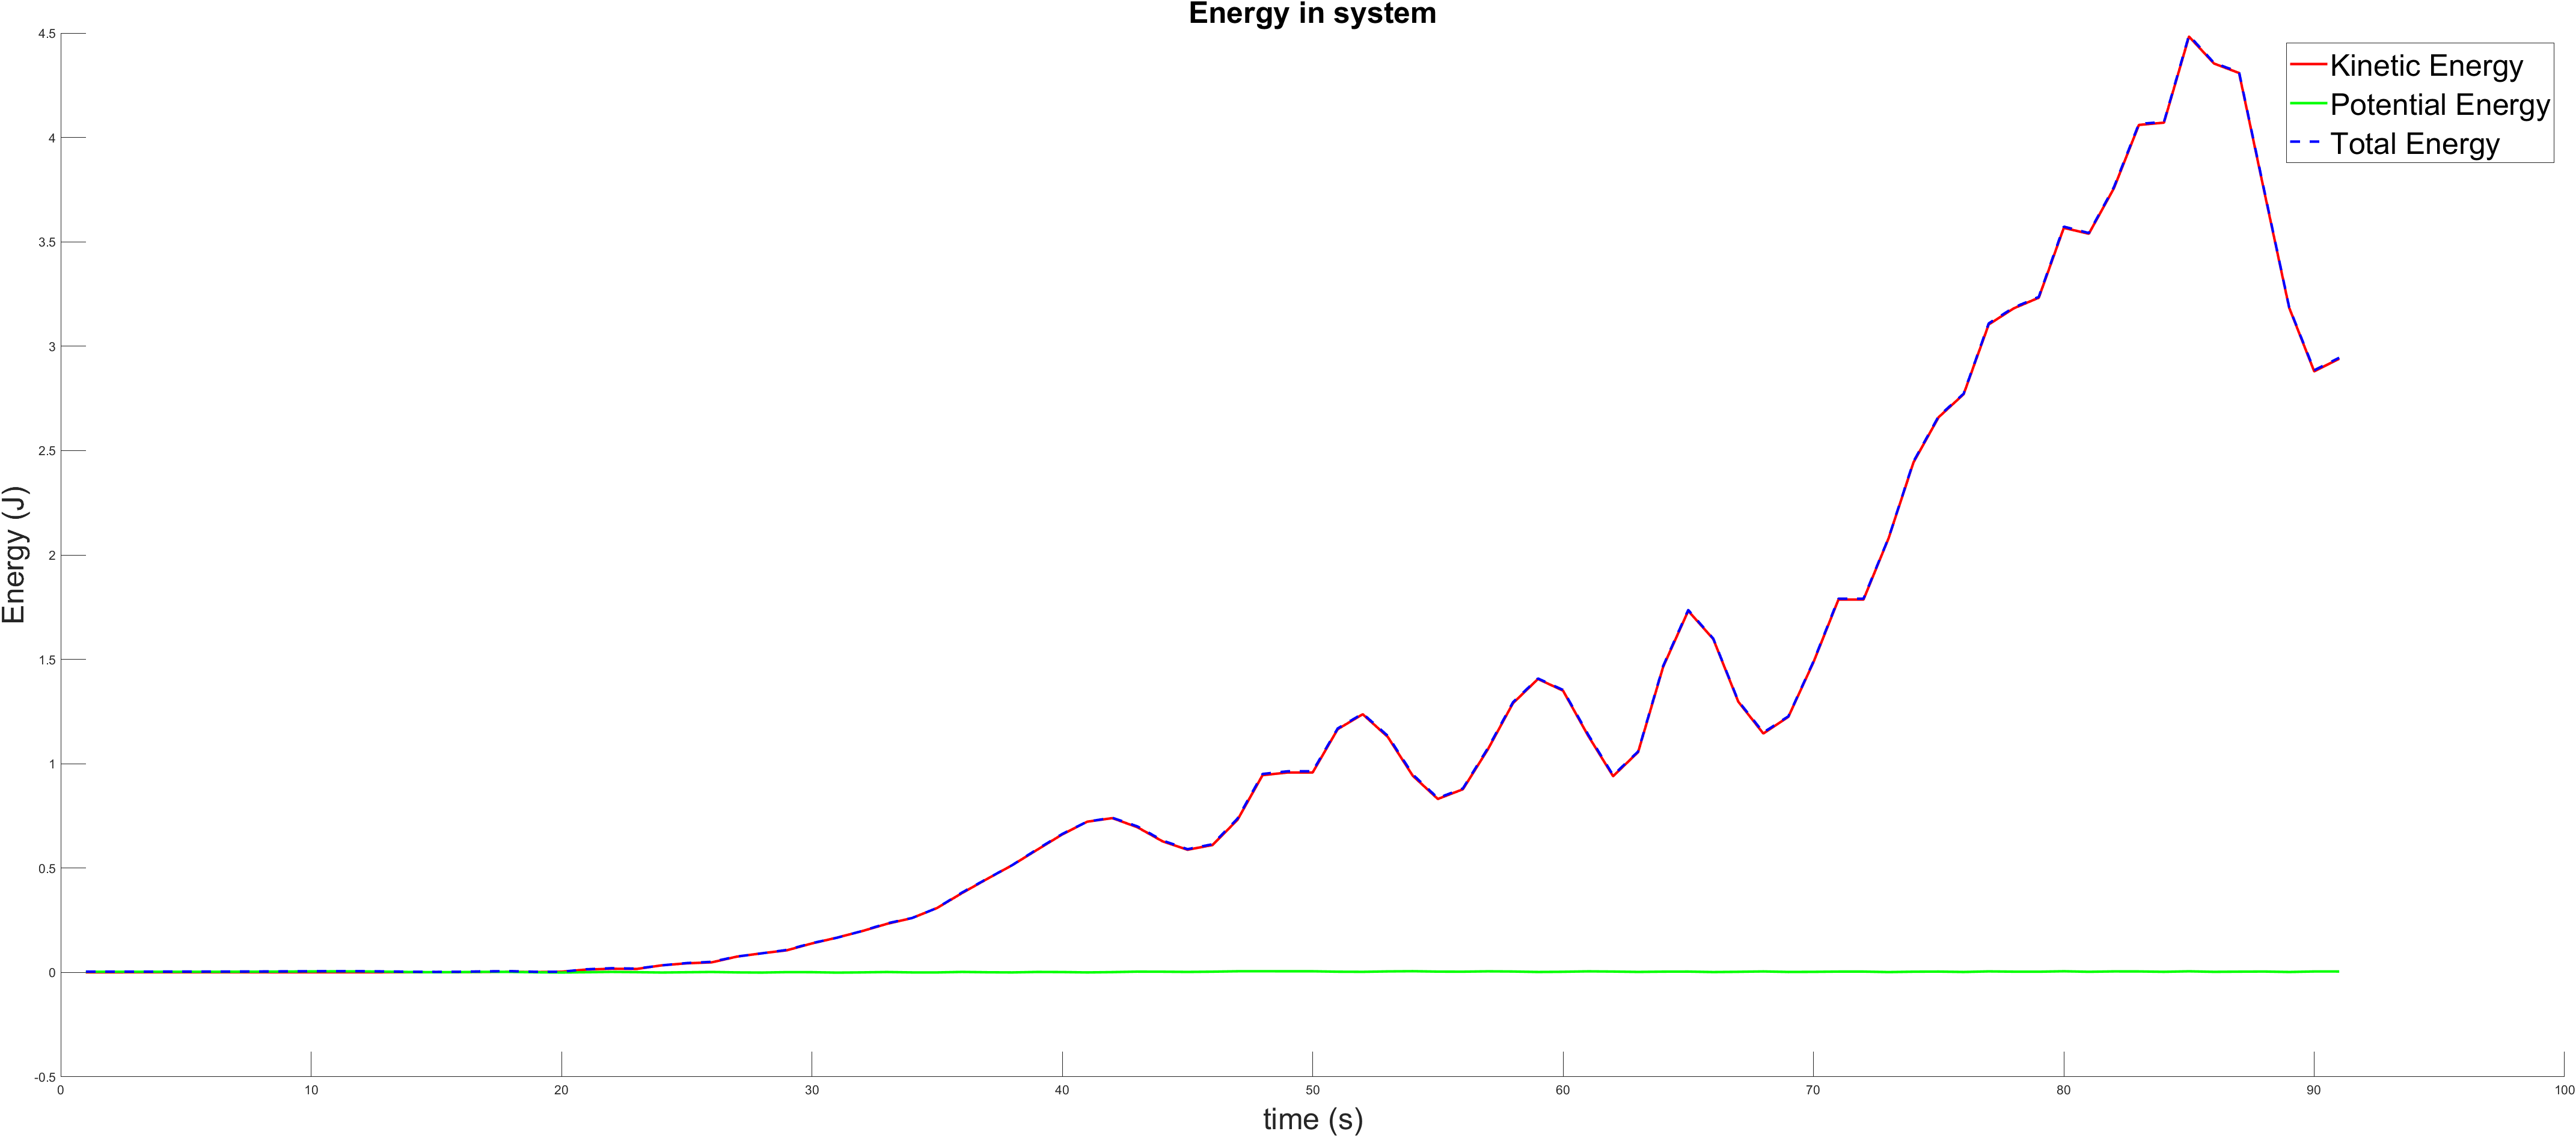
\includegraphics[width=15cm]{Energy_analysis}
		\caption{Energy Plot for my system}%
	\end{figure}
\end{center}

\section{Appendix}
\subsection{The Lagrangian}
\[
\begin{aligned}
	& \mathcal{L} = \frac{m_4}{2}\bigl((\dot{x}_g + 2d_1\dot{\theta}_1\cos(\theta_1) + 2d_2\dot{\theta}_2\cos(\theta_2) 
	+ d_3\dot{\theta}_3\cos(\theta_3))^2 \\
	&\qquad + (\dot{y}_g + 2d_1\dot{\theta}_1\sin(\theta_1) + 2d_2\dot{\theta}_2\sin(\theta_2) 
	+ d_3\dot{\theta}_3\sin(\theta_3))^2 \bigr) \\
	&\quad + g\bigl(m_3(2d_1\cos(\theta_1) - y_g + d_2\cos(\theta_2)) 
	- m_2(y_g - d_1\cos(\theta_1)) - m_1y_g \\
	&\qquad + m_4(2d_1\cos(\theta_1) - y_g + 2d_2\cos(\theta_2) + d_3\cos(\theta_3))\bigr) \\
	&\quad + \frac{m_2}{2}\bigl((\dot{x}_g + d_1\dot{\theta}_1\cos(\theta_1))^2 
	+ (\dot{y}_g + d_1\dot{\theta}_1\sin(\theta_1))^2\bigr) \\
	&\quad + \frac{m_1}{2}(\dot{x}_g^2 + \dot{y}_g^2) \\
	&\quad + \frac{m_3}{2}\bigl((\dot{x}_g + 2d_1\dot{\theta}_1\cos(\theta_1) + d_2\dot{\theta}_2\cos(\theta_2))^2 
	+ (\dot{y}_g + 2d_1\dot{\theta}_1\sin(\theta_1) + d_2\dot{\theta}_2\sin(\theta_2))^2\bigr) \\
	&\quad + \frac{d_1^2 m_2 \dot{\theta}_1^2}{6} 
	+ \frac{d_2^2 m_3 \dot{\theta}_2^2}{6} 
	+ \frac{d_3^2 m_4 \dot{\theta}_3^2}{6}.
\end{aligned}
\]

\end{document}  


